\subsection{Define Algorithm}

Normally, the algorithms used to calculate the electricity consumption depend on a large amount of variables and factors, as can be seen on figure 7: \citep{costa2012} \\

\begin{figure}[htb!]
	\centering
	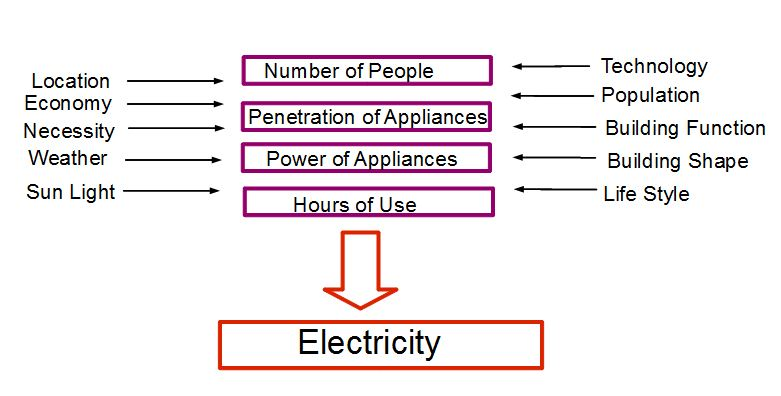
\includegraphics[width=0.8\textwidth]{phase2/group3/fig8.png}
	\caption{Factors for calculating the electricity consumption (Costa, 2012) }
	\label{fig:figure8}
\end{figure}

According to this sketch, in order to calculate the electricity consumption, except the number of people, it is required to know the penetration of appliances, the power of appliances and the hours of use. Such data are changed from one situation to another. The available data cannot support this algorithm, and, therefore, some assumptions are done in order to simplify the process.

According to this situation, a new algorithm is created to estimate the annual consumption based on different household. Figure 9 illustrates the annual consumption for different number of household. Since the number of apartment and residents in each building already calculated in Phase I. If  the residents can be distributed into each apartment as household, the electricity consumption can be calculated from it.

\begin{figure}[H]
	\centering
	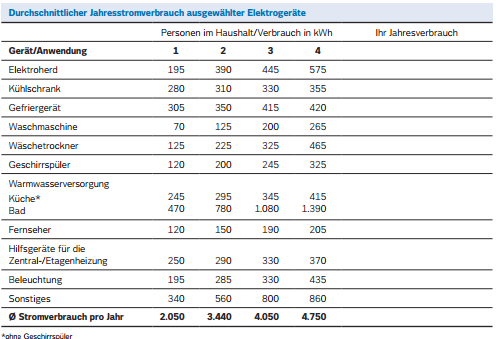
\includegraphics[width=0.8\textwidth]{phase2/group3/fig9.png}
	\caption{The annual electricity consumption for different number of household (Vattenfall 2012) }
	\label{fig:figure9}
\end{figure}

\subsection{Data Source}
From Phase I, the results are mainly two indicators: Apartments/volume and Resident/ Building. If these two indicators are applied to all the residential buildings, the number of apartments per buildings will be get. Also the average share of household in Mitte can be found in statistic department.\citep{statsberlin} Combining the electricity consumption data from Vattenfall, all the data for estimating the annual consumption is provided.

\subsection{Method}
Figure 8 illustrates the work flow for calculate the results as well the data sources:

\begin{figure}[htb!]
	\centering
	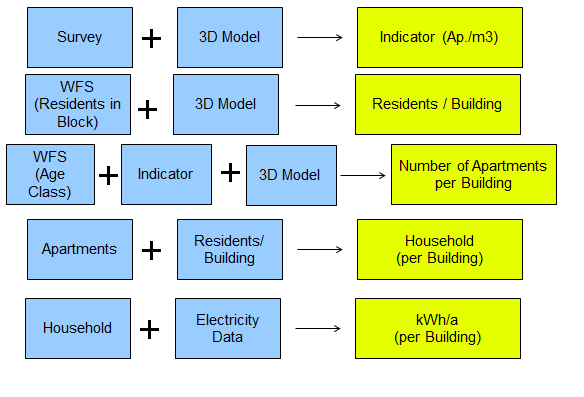
\includegraphics[width=0.6\textwidth]{phase2/group3/fig10.png}
	\caption{Workflow for Phase II }
	\label{fig:figure10}
\end{figure}

For the last step, there are two ways to calculate the electricity:
1) Establish the regression equation and apply the average household in the equation (see figure 10). This equation was created from the data available on Figure 8.

\begin{figure}[H]
	\centering
	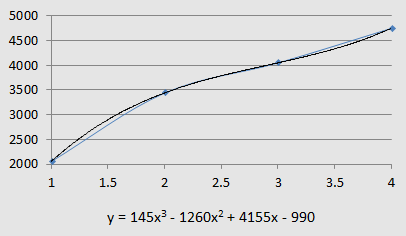
\includegraphics[width=0.6\textwidth]{phase2/group3/fig11.png}
	\caption{The regression equation for electricity consumption}
	\label{fig:figure11}
\end{figure}

2) Distribute the residents into each apartment to get the number of apartment with different household. And use these numbers to multiply the corresponding electricity and lighting consumption. This distribution is base on the statistical share of households for the giving area.

\subsection{Household Distribution}
One of the most important parts in the second method is distributing the inhabitants into apartment. There are three inputs already known: the apartment number, the residents number and the average share of different household. To distribute the residents, only two variables above can be fixed with one variable left. Therefore there are three methods: 

\begin{itemize}
\item Fix the share and residents number, take apartment number as variable
\item Fix the share and apartment number, take residents number as variable
\item Fix the apartment and residents number, take share as variable
\end{itemize}

While for the first two methods the variable parameters will be changed in a unreasonable way, and make the results not reliable, a new distribution method is developed from the third method. 

\subsubsection{Basic Idea}
The basic idea of this method is to try to keep the share close to the average share of Mitte, by applying the following steps:\\
\\
1. Spit the total number of apartment with different household based on the percentage \\
2. Check how many residents left\\
3. Distribute the left residents\\
4. Keep the ratio of the 2~4 household: 3:1:1

\subsubsection{First Distribution}
After the first distribute based on the share, there will be three difference scenes:\\
\begin{itemize}
\item $R > 0$   more people live in one apartment
\item $R < 0$   less people live in one apartment
\item $R < Apartment$  only household(1) and empty apartment
\end{itemize}

In the last scenes, all residents will be put into each apartment with only 1 household and the other apartments are empty. For the first and second scenes, the left residents have to be distributed again.

\subsubsection{Second Distribution}
In the second distribution, as can be seen in figure 11, if only one residents left, it will be put into an apartment with 1 household, which means the number of 1 household will decrease 1 and the number of 2 household will increase 1. If two left, put both of them into 1 household. And the number of 1 household will also decrease 1 but the number of 3 household will increase 1. Do the same as shown in the figure 11 until 8. if there are 9 left, distribute the first 8 as -5:3:1:1 then put the left 1 to 1 household. \\
By this distribution method, it keeps the ratio of the 2~4 household as 3:1:1, which also means every 8 residents as a loop. 


\begin{figure}[H]
	\centering
	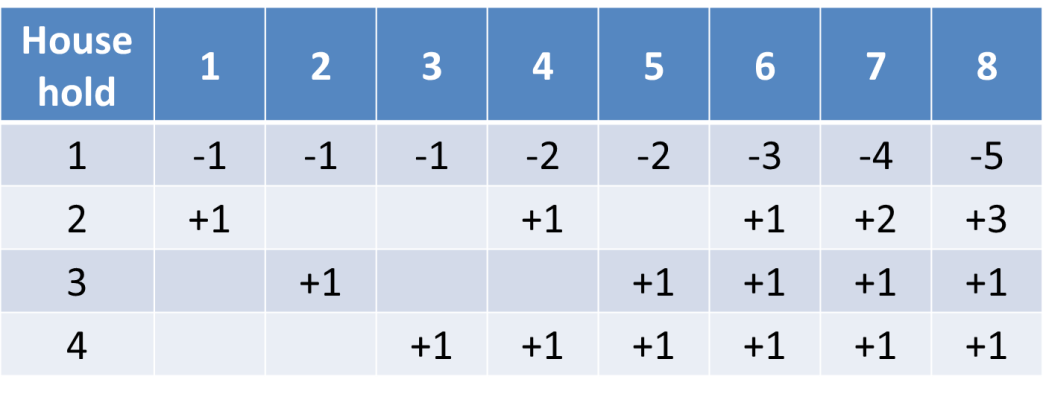
\includegraphics[width=0.8\textwidth]{phase2/group3/fig12.png}
	\caption{The second residents’ distribution method (Self Made)}
	\label{fig:figure12}
\end{figure}

\subsection{ArcPython User Interface}

To apply this method to other dataset, an Arctool was designed by using python script which has a good connection with ArcGIS 10. 

\begin{figure}[ht]
	\centering
	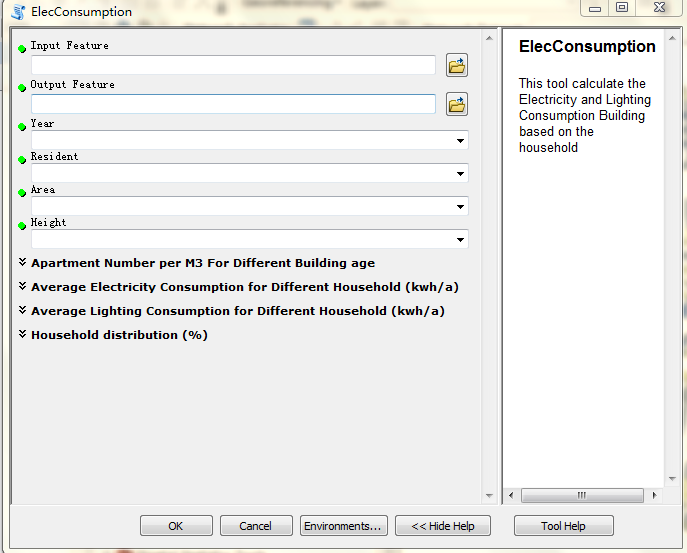
\includegraphics[width=0.8\textwidth]{phase2/group3/fig13.png}
	\caption{Developed Arctool (Self Made)}
	\label{fig:figure13}
\end{figure}


\begin{figure}[H]
	\centering
	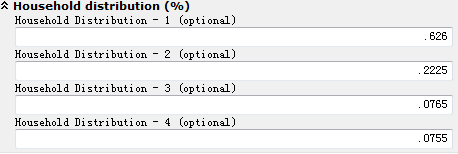
\includegraphics[width=0.8\textwidth]{phase2/group3/fig14.png}
	\caption{Developed Arctool - State Variables (Self Made)}
	\label{fig:figure14}
\end{figure}

The user can choose the input and output feature class and select the corresponding fields for building age, residents, area and height to calculate the electricity consumption. Besides, the user can also change the optional parameters such as the share of household and the annual electricity consumption for different household.

\subsection{Results}
After the resident distribution, the light and electricity consumption can be computed by multiplying the number of apartment with different household with corresponding consumption

\begin{figure}[ht]
	\centering
	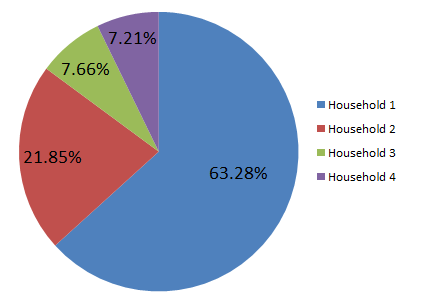
\includegraphics[width=0.7\textwidth]{phase2/group3/fig15.png}
	\caption{Final Household Share (Self Made)}
	\label{fig:figure15}
\end{figure}

\begin{figure}[ht]
	\centering
	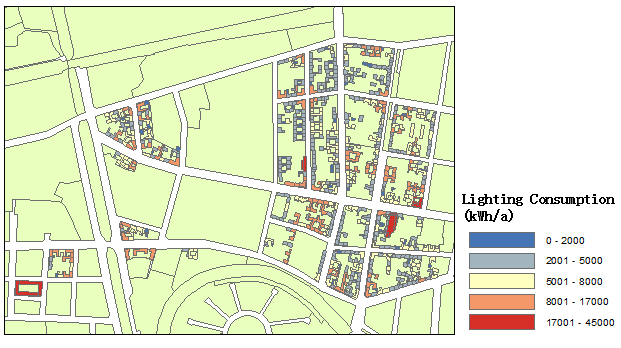
\includegraphics[width=1\textwidth]{phase2/group3/fig16.png}
	\caption{Final Lighting Consumption (Self Made)}
	\label{fig:figure16}
\end{figure}

\begin{figure}[H]
	\centering
	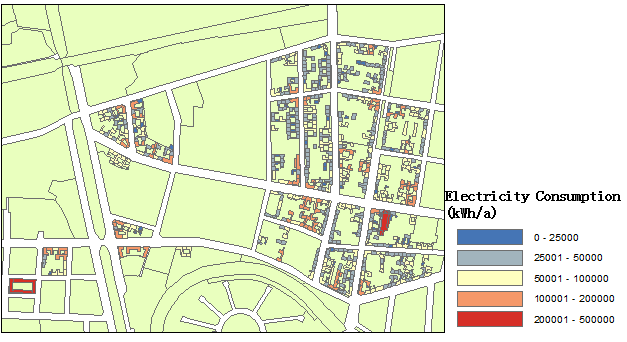
\includegraphics[width=1\textwidth]{phase2/group3/fig17.png}
	\caption{Final Electricity Consumption (Self Made)}
	\label{fig:figure17}
\end{figure}
\begin{figure}[H]
	\centering
	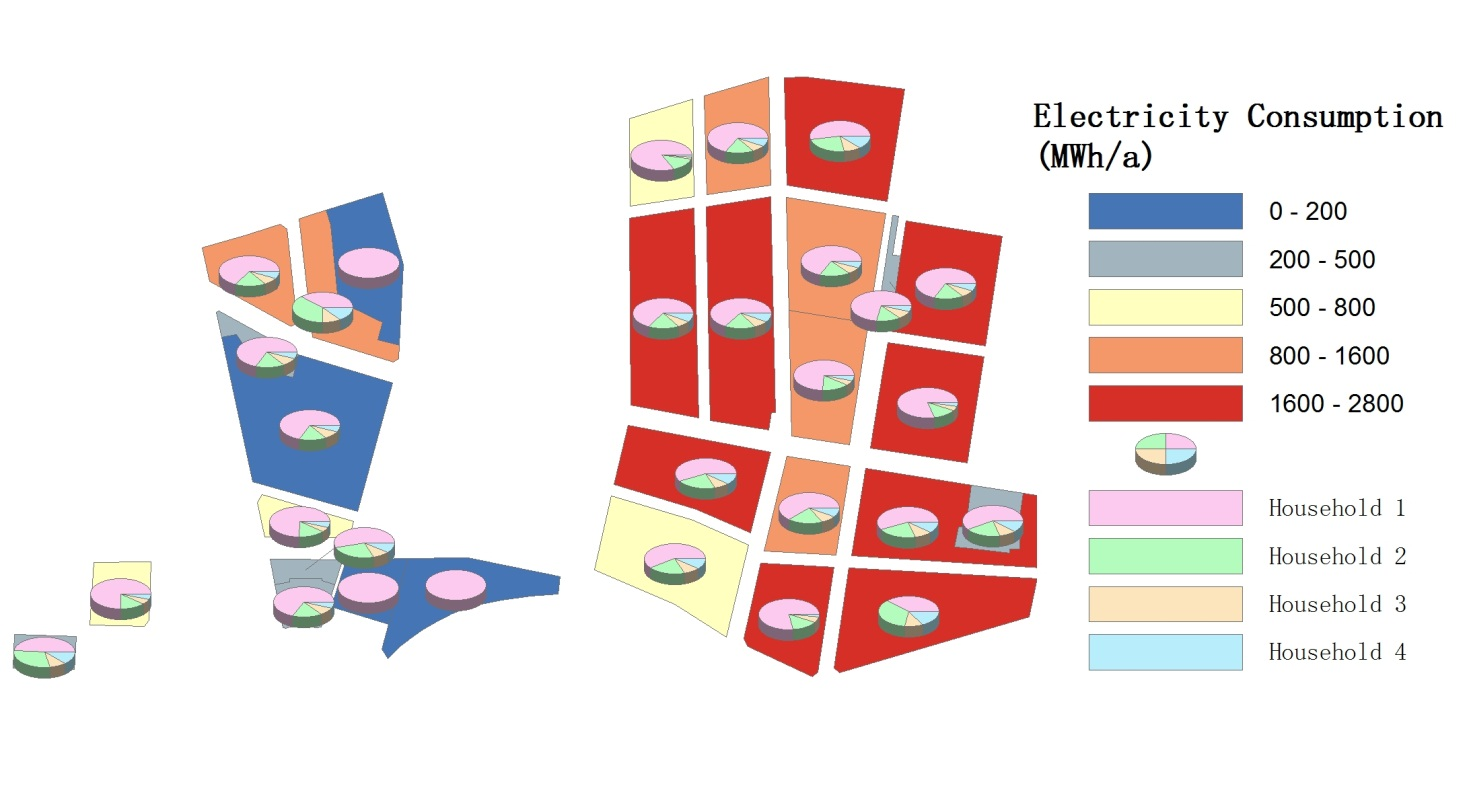
\includegraphics[width=0.9\textwidth]{phase2/group3/fig19.png}
	\caption{Final Electricity Consumption per Block (Self Made)}
	\label{fig:figure19}
\end{figure}
Table 2 shows the results from the two calculation methods. As can be seen from it, using the average household and regression equation the results are smaller than the distribution method. Nevertheless, both estimation methods rendered values within a short interval - as both are based essentially on the residents per building and/or per apartment. 


\begin{table}[H]
	\centering
	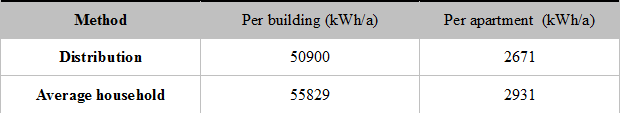
\includegraphics[width=0.8\textwidth]{phase2/group3/fig18.PNG}
	\caption{Final Electricity Consumption (Self Made)}
	\label{fig:figure18}
\end{table}



\subsection{Conclusion}
The described method is able to integrate statistical data, surveying data and virtual 3D City Models. Furthermore, it provides a rough tool to calculate the electricity for other area which can be implemented in 3D City Models. As a result, instead of having only average results, the calculations are also locally performed. In other words, as the parameters are first calculated per each building, it is also possible to select the final results for each building. The two distribution methods provide the user two different level results with different data. If there is no household share data, the regression equation method can give the rough results. While with the household share data, the distribution method can be applied for more reasonable results.\\

The 3D Model is able to provide all the demanded geometrical factors. Once the electricity consumption estimation is geometrically based on the volume of the buildings, data regarding its footprint area and height are required. \\

However, there still some parts need to pay attention to during applying this method. Such as the function of the building, the relationship between 3D City Model and the survey address.
